\documentclass{standalone}
\usepackage{tikz}
\usetikzlibrary{arrows.meta}


\tikzstyle{input-node}=[fill=white,circle,thick,draw]
\tikzstyle{hidden-node}=[fill=white,circle,thick,draw]
\tikzstyle{output-node}=[fill=white,circle,thick,draw]
\tikzstyle{empty-node}=[fill=white,circle]

\tikzstyle{black-line}=[draw=black,very thick]
\tikzstyle{red-line}=[draw=red,very thick]

\begin{document}
	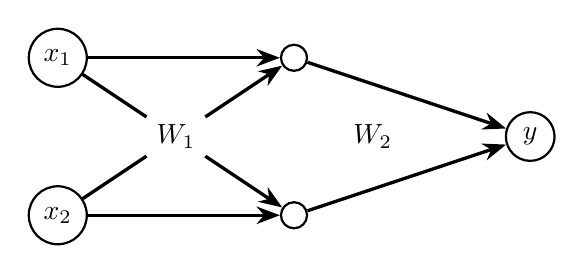
\begin{tikzpicture}
	\begin{scope}
	\node (i1)[input-node] at (0,2) {$x_1$};
	\node (i2)[input-node] at (0,0) {$x_2$};
	
	
	\node (h1)[hidden-node] at (3,2) {};
	\node (h2)[hidden-node] at (3,0) {};
	
	\node (o1)[output-node] at (6,1) {$y$};
	\end{scope}
	
	\begin{scope}[>={Stealth[black]}, every edge/.style=black-line]
	\path [->] (i1) edge node {} (h1);
	\path [->] (i1) edge node {} (h2);
	\path [->] (i2) edge node {} (h1);
	\path [->] (i2) edge node {} (h2);
	\path [->] (h1) edge node {} (o1);
	\path [->] (h2) edge node {} (o1);
	\end{scope}
	
	\begin{scope}
	\node (w1)[empty-node] at (1.5,1) {$W_1$};
	\node (w2)[empty-node] at (4,1) {$W_2$};
	\end{scope}
	\end{tikzpicture}
\end{document}